\documentclass{article}

\usepackage[utf8]{inputenc}
\usepackage{amsmath,amssymb,amsfonts,amsthm}
\usepackage{graphicx}
\usepackage{listings}
\usepackage{xcolor}
\usepackage{booktabs}
\usepackage{microtype}
\usepackage{tabularx}
\usepackage{enumitem}
\usepackage{caption}
\usepackage{colortbl}
\usepackage{placeins}
\usepackage{hyperref}

\usepackage{mlsys2025}

% the bibliography is numeric; the style defaults to author-year
\setcitestyle{numbers,square}

\mlsystitlerunning{KernelLens: Recovering the Triton-to-C++ Engine Contract}

\graphicspath{{docs/assets/figures/}{./}}

\definecolor{primaryblue}{RGB}{24, 76, 120}
\definecolor{backcolour}{rgb}{0.97,0.97,0.97}
\definecolor{codegreen}{rgb}{0,0.5,0}
\definecolor{codegray}{rgb}{0.5,0.5,0.5}
\definecolor{codepurple}{rgb}{0.58,0,0.82}
\definecolor{bordergray}{rgb}{0.85,0.85,0.85}

\hypersetup{colorlinks=true, linkcolor=primaryblue, citecolor=primaryblue, urlcolor=primaryblue}
\emergencystretch=6em

\lstdefinestyle{mystyle}{
    backgroundcolor=\color{backcolour},
    commentstyle=\color{codegreen},
    keywordstyle=\color{primaryblue}\bfseries,
    numberstyle=\tiny\color{codegray},
    stringstyle=\color{codepurple},
    basicstyle=\ttfamily\tiny,
    breaklines=true, captionpos=b, keepspaces=true,
    numbers=left, numbersep=5pt,
    showspaces=false, showstringspaces=false, showtabs=false,
    tabsize=2, frame=single, rulecolor=\color{bordergray}
}
\lstset{style=mystyle}
\newcommand{\code}[1]{\texttt{#1}}

\title{dummy}
\date{dummy}

\begin{document}
\twocolumn[
\mlsystitle{KernelLens: Recovering the Triton-to-C++ Engine Contract}

\begin{mlsysauthorlist}
\mlsysauthor{Justin Duc}{galiad}
\end{mlsysauthorlist}

\mlsysaffiliation{galiad}{Galiad Research}
\mlsyscorrespondingauthor{Justin Duc}{justin.duc@galiad-research.com}

\vskip 0.3in



\begin{abstract}
OpenAI Triton has become the standard way to author custom GPU kernels, and
NVIDIA TensorRT and Microsoft ONNX Runtime the standard way to serve models in
C++. The two do not compose. A compiled Triton kernel is a self-contained
artifact, but the interface between it and a C++ engine---how the kernel's
parameters map onto the engine's tensors, how its launch grid is evaluated, and
which of its arguments alias---is implicit and undocumented.

We present \textbf{KernelLens}, which recovers that interface automatically from
the compiled artifacts and re-establishes it as native TensorRT and ONNX Runtime
plugins. The recovery has three parts: (i)~parsing the PTX entry signature to
rebuild the host argument array that Triton's backend re-ordered, dropped and
re-bitwidth'd; (ii)~capturing the launch grid symbolically and transpiling it to
C++ evaluated at run time; and (iii)~classifying each argument as input, output
or in-place by static AST analysis, including through nested helper functions.
Re-establishing the interface \emph{inside} the ONNX graph lets the engine keep
its graph optimisations around the plugin. The result replaces $1{,}137$~lines
of hand-written C++ --- measured, not estimated, on one fused RMSNorm kernel
built for both backends --- with two Python calls. On an
RTX~5060~Ti, KernelLens reproduces native Triton exactly on ten research
workloads and fourteen module patterns, and on a block whose attention is a
custom squared-ReLU flash kernel it is $1.99\times$ faster than the folded-only
formulation and $1.08\times$ faster than the unfused kernel path.
\end{abstract}
]

\printAffiliationsAndNotice{}


\section{Introduction}

Two mature technologies meet awkwardly at deployment. On one side, OpenAI Triton
\cite{triton2019} has become the standard way to write custom GPU kernels in
Python: a \texttt{@triton.jit} function is compiled to PTX and launched from
Python. On the other, production inference is served by C++ engines---NVIDIA
TensorRT \cite{tensorrt} and Microsoft ONNX Runtime \cite{onnxruntime}---which
apply whole-graph optimisation, kernel selection and VRAM planning. A model that
calls a Triton kernel fits neither: the exporter cannot trace the kernel, and the
engine has no way to execute it.

The usual reading of this problem is that Triton and the engines are
incompatible. We argue the opposite, and that is the thesis of this paper:

\begin{quote}
\textbf{A compiled Triton kernel is a complete, self-contained artifact. The
interface between it and a C++ engine is implicit and undocumented, but it can be
recovered automatically.}
\end{quote}

Once recovered, the interface can be \emph{re-established} on the engine's terms:
the kernel becomes a native custom operator, and---because it is injected into
the graph rather than around it---the engine continues to fold and tune the
standard layers. The result is a model that keeps both the engine's graph
optimisations and its custom kernels.

\paragraph{What is new.} The contribution is not a new algorithm; it is a
capability that did not previously exist, enabled by three recovery techniques:

\begin{enumerate}[leftmargin=1.6em]
    \item \textbf{PTX entry-signature recovery.} Triton's backend re-orders,
    drops and re-bitwidths the parameters relative to the Python signature. We
    parse the PTX \texttt{.entry} declaration, map its slots back onto the
    kernel's arguments, and rebuild the host \texttt{void*[]} launch array. This
    is the step that lets the \emph{already compiled} kernel run inside TensorRT
    or ONNX Runtime without being rewritten in CUDA.
    \item \textbf{Symbolic launch-grid capture and C++ transpilation.} The grid
    is a Python expression over runtime shapes; we recover it with a dual-pass
    tracer and transpile it into C++ integer arithmetic evaluated at inference
    time.
    \item \textbf{Static AST argument taxonomy.} Classifying each argument as
    input, output or in-place---including through nested \texttt{@triton.jit}
    helpers---is what allows the ONNX graph to be wired correctly.
\end{enumerate}

\paragraph{Contributions.}
\begin{enumerate}[leftmargin=1.6em]
    \item The recovery techniques above, integrated into a compile pipeline that
    turns an unmodified \texttt{torch.nn.Module} into an ONNX graph plus TensorRT
    and ONNX Runtime plugin libraries (\S\ref{sec:recover}, \S\ref{sec:reestablish}).
    \item A run pipeline that binds PyTorch GPU addresses directly to both engines
    with no host staging (\S\ref{sec:reestablish}).
    \item An empirical study---parity, module-pattern coverage, folding plus
    kernels, latency, end-to-end and quantized results---showing that the
    composition is correct and that keeping the kernel while folding the rest is
    faster than either alone (\S\ref{sec:eval}).
\end{enumerate}

\section{Related Work}
\label{sec:related}

\paragraph{GPU kernel languages.} Triton \cite{triton2019} lowers a Python DSL to
PTX through its own LLVM backend, choosing tiling, vectorisation and shared-memory
use. It is the substrate this paper deploys; we treat the compiled artifact as
given and recover its interface rather than recompiling it. Halide
\cite{halide} and TVM \cite{tvm} take the complementary route of scheduling from
a computation description. MLIR \cite{mlir} provides the dialect infrastructure
that many of these systems share.

\paragraph{Compilers that lower PyTorch.} \texttt{torch.compile}, backed by
TorchInductor \cite{pytorch20}, generates Triton for eager PyTorch graphs and is
the natural performance baseline. It runs inside a Python process and depends on
\texttt{libtorch}; it emits neither a standalone ONNX graph nor a C++ plugin for
a non-Python server. AOTInductor \cite{aotinductor} produces shared libraries but
still links the PyTorch C++ runtime. Since PyTorch~2.1, \texttt{torch.compile}
also \emph{captures} user Triton kernels---TorchDynamo records a
\texttt{triton\_kernel\_wrapper\_mutation} node with no graph break, and
Inductor emits a call to the user's kernel---which makes it a strong in-process
baseline, but not a deployment path.

\paragraph{Inference engines and custom operators.} TensorRT \cite{tensorrt} and
ONNX Runtime \cite{onnxruntime} expose C++ extension points
(\texttt{nvinfer1::IPluginV2DynamicExt} with \texttt{IPluginCreator}, and
\texttt{OrtCustomOp}) and drive execution themselves, handing operators raw device
pointers. KernelLens synthesises these; the graph-level value of doing so is
shared with serving systems such as vLLM \cite{vllm} and TensorRT-LLM
\cite{tensorrt_llm}, which likewise fuse standard layers and dispatch custom
kernels from a C++ runtime.

\paragraph{Triton kernel libraries.} Liger-Kernel \cite{ligerkernel},
FlashAttention \cite{flashattn1,flashattn2} and AOTriton supply high-quality
kernels. KernelLens is the deployment layer beneath such libraries: it does not
compete on kernel quality, it makes an existing kernel deployable.

\paragraph{Positioning.} The distinguishing property is the combination of
automated PyTorch graph export \emph{and} self-contained C++ plugins for both
engines, from the compiled Triton artifact, with no manual C++ and no CUDA
rewrite.

\section{The Manual Pipeline}
\label{sec:manual}

Before the recovery, it is worth being concrete about what it replaces.
Figure~\ref{fig:manual} (top) is the pipeline a developer builds by hand to put
one Triton kernel into either engine. It splits into a compile side and two run
lanes.

\begin{figure*}[t]
\centering
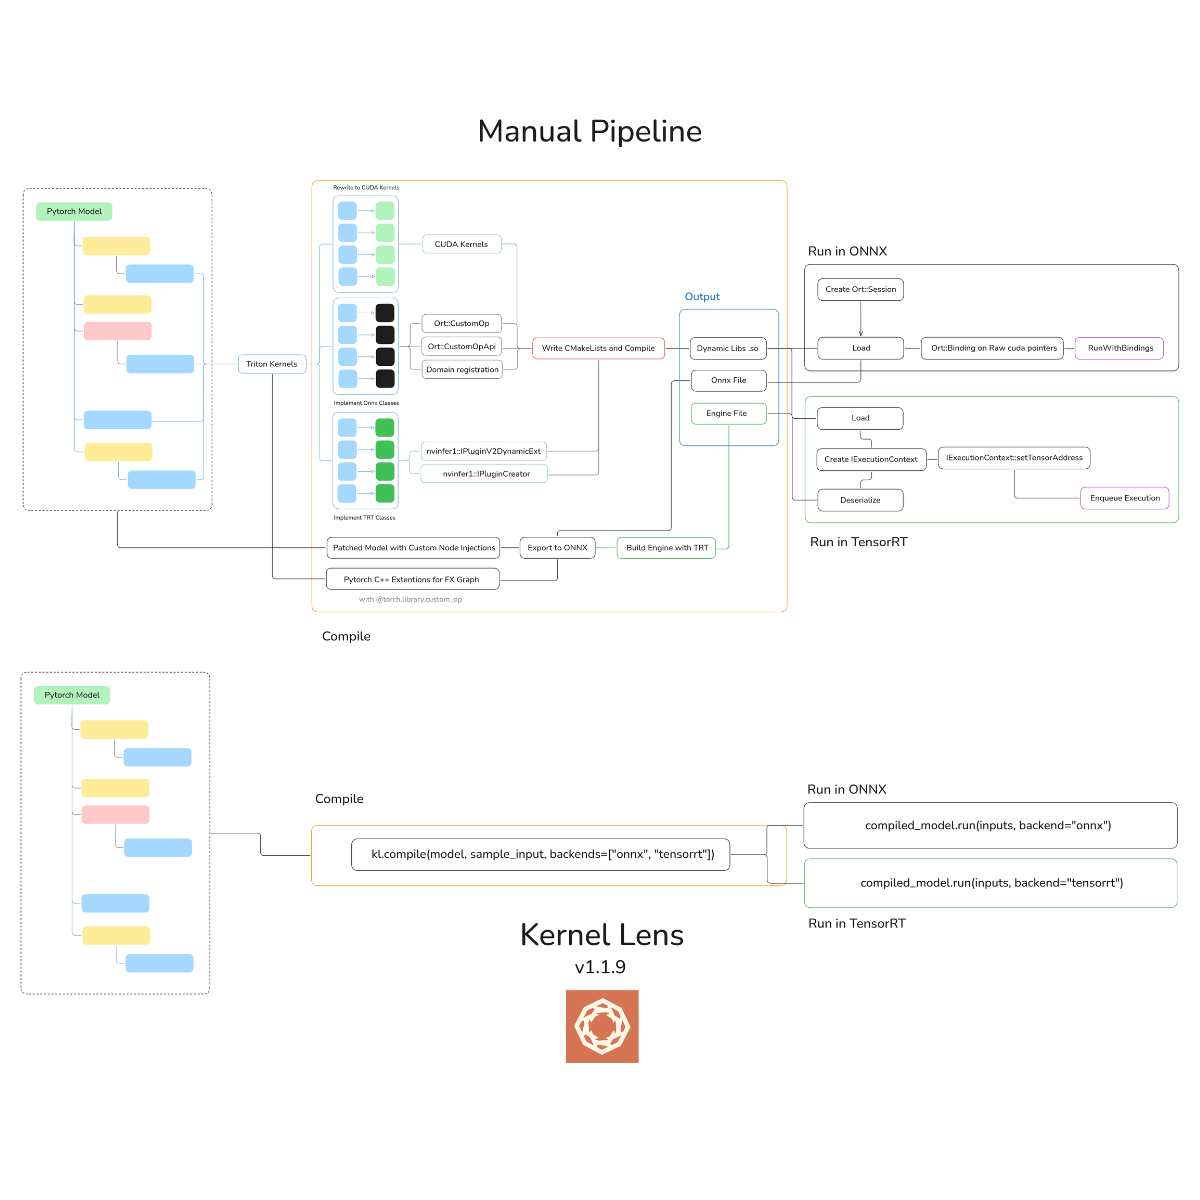
\includegraphics[width=0.78\textwidth]{architectural_diagram.png}
\caption{Top: the manual pipeline. Every box is a class, a build step or an
engine call written and maintained by hand---rewriting the kernel in CUDA,
\texttt{Ort::CustomOp}, \texttt{Ort::CustomOpApi}, domain registration,
\texttt{IPluginV2DynamicExt}, \texttt{IPluginCreator}, CMake, FX-graph patching
with \texttt{@torch.library.custom\_op}, ONNX export, TensorRT engine building,
\texttt{RunWithBindings} and \texttt{Enqueue Execution}. Bottom: KernelLens.}
\label{fig:manual}
\end{figure*}

\paragraph{Compile.} (1)~Port the kernel to CUDA C++. (2)~Implement the ONNX
Runtime classes: derive from \texttt{OrtCustomOp}, use \texttt{Ort::CustomOpApi}
to read inputs, write outputs and launch, and register a schema and domain.
(3)~Implement the TensorRT classes: \texttt{getOutputDimensions},
\texttt{supportsFormatCombination}, \texttt{enqueue} and serialization, plus an
\texttt{IPluginCreator}. (4)~Write CMakeLists, drive \texttt{nvcc} and
\texttt{g++}, resolve the ORT and TensorRT headers. (5)~Patch the FX graph
through a C++ extension, wrap each kernel with
\texttt{@torch.library.custom\_op}, and inject the nodes before export.
(6)~Produce the artifacts: a shared library, an ONNX file and a TensorRT engine.

\paragraph{Run.} ONNX Runtime: create an \texttt{Ort::Session}, load the library,
bind raw CUDA pointers through \texttt{Ort::Binding}, call
\texttt{RunWithBindings}. TensorRT: deserialize the engine into an
\texttt{IExecutionContext}, call
\texttt{IExecutionContext::setTensorAddress} for every tensor, enqueue.

Each step is a place where the ABI, the launch geometry, the memory placement or
the numerics can diverge from the original kernel.

\FloatBarrier
\section{The Triton-to-Engine Contract}
\label{sec:contract}

The recovery is only possible because a compiled Triton kernel carries more
information than its Python signature suggests. We formalise what a kernel
presents as
\begin{equation}
\mathcal{K} = \big\langle \mathbf{P}_{\text{in}}, \mathbf{P}_{\text{out}},
\mathbf{P}_{\text{inplace}}, \mathbf{S}, \mathbf{D}, \mathbf{C}, \mathbf{G} \big\rangle,
\end{equation}
where $\mathbf{P}_{\text{in}}$, $\mathbf{P}_{\text{out}}$ and
$\mathbf{P}_{\text{inplace}}$ are read-only, write-only and read--write VRAM
pointers; $\mathbf{S}$ are element strides; $\mathbf{D}$ are dynamic host scalars;
$\mathbf{C}$ are \texttt{tl.constexpr} values baked into PTX; and $\mathbf{G}$ is
the launch grid, computed from runtime dimensions.

\begin{table*}[t]
\centering
\small
\begin{tabularx}{\textwidth}{l l X}
\toprule
\textbf{Component} & \textbf{Meaning} & \textbf{Mechanism in the engine} \\ \midrule
$\mathbf{P}_{\text{in}}$ & read-only pointers & operator inputs, bound by address \\
$\mathbf{P}_{\text{out}}$ & write-only pointers & operator outputs, engine-allocated \\
$\mathbf{P}_{\text{inplace}}$ & read and written & input/output aliasing \\
$\mathbf{S}$ & element strides & \texttt{int64} runtime arguments \\
$\mathbf{D}$ & per-call scalars & CPU inputs / plugin members \\
$\mathbf{C}$ & \texttt{tl.constexpr} & baked in PTX, absent from the ABI \\
$\mathbf{G}$ & launch grid & C++ integer expression evaluated at run time \\
\bottomrule
\end{tabularx}
\caption{The seven components of the contract and the engine mechanism each maps to.}
\label{tab:contract}
\end{table*}

Two of these are why a naive export fails. The PTX entry signature is Triton's,
not the programmer's: parameters are re-ordered, unused ones are dropped, and
widths are fixed. And the grid is an arbitrary Python expression over runtime
shapes. Neither is recoverable from the Python source alone; both are recoverable
from the compiled artifacts.

\section{Recovering the Contract}
\label{sec:recover}

KernelLens observes the model twice and inspects the kernel source once. The
three passes produce a \texttt{KernelManifest}, the structured form of the
contract.

\subsection{Pass 1: the compiled artifact}

The model runs once on the GPU while \texttt{triton.JITFunction.run} is patched.
For each launch KernelLens reads the compiled PTX, the dynamic shared-memory
size, \texttt{num\_warps}, the real launch grid, and every argument's shape,
strides and dtype. This is the only pass that sees the true compiled artifact, so
it is the source of the PTX and the concrete tensor metadata.

\subsection{Pass 2: the symbolic grid}

The module is re-executed under \texttt{make\_fx(tracing\_mode="symbolic")} with
fake tensors, so the grid lambda evaluates over \texttt{SymInt} sizes. The
resulting expression---for example \texttt{(s0*s1+127)//128}---is captured as a
string for later transpilation. If this pass diverges from Pass~1, the concrete
manifests are used unchanged, which keeps compilation deterministic.

\subsection{Pass 3: the argument taxonomy}

An \texttt{ast.NodeVisitor} walks the kernel source, recursively into
\texttt{@triton.jit} helper functions that are called, and records every
\texttt{tl.load} and \texttt{tl.store} target. An argument that appears in both
sets is \texttt{inplace}; one that is only stored is \texttt{output}; the rest are
\texttt{input}. This is what tells the graph which buffers alias and which scalars
must be per-call CPU inputs.

\subsection{PTX entry-signature recovery}

The central technique is reconstructing the host ABI. Triton emits an
\texttt{.entry} declaration whose parameters do not correspond to the Python
signature. KernelLens parses it, determines each slot's C type (\texttt{void*},
\texttt{int64\_t}, \texttt{float}, \texttt{int32\_t}) and its textual parameter
number, and maps the slots back onto the manifest's arguments. The launch
argument array is then rebuilt to match the PTX exactly. Table~\ref{tab:recovery}
lists what is recovered and from where.

\begin{table*}[t]
\centering
\small
\begin{tabularx}{\textwidth}{l X}
\toprule
\textbf{Recovered} & \textbf{From} \\ \midrule
Parameter order, count and bitwidths & \texttt{.entry <kernel> (.param ...)} in the PTX \\
Entry function name (mangled) & \texttt{.visible .entry <name>} \\
Block size & \texttt{.reqntid} \\
Shared-memory size & the compiled kernel's metadata \\
Launch grid & the symbolic pass (Pass~2) \\
Input / output / in-place & the AST scan (Pass~3) \\
\bottomrule
\end{tabularx}
\caption{Each component of the contract and the artifact it is recovered from.}
\label{tab:recovery}
\end{table*}

\section{Re-establishing the Contract}
\label{sec:reestablish}

With the contract in hand, KernelLens rebuilds it on the engine's terms. One call
does the whole thing:
\texttt{kl.compile(model, sample\_input, backends=[...])}
(Figure~\ref{fig:compile}).

\begin{figure*}[t]
\centering
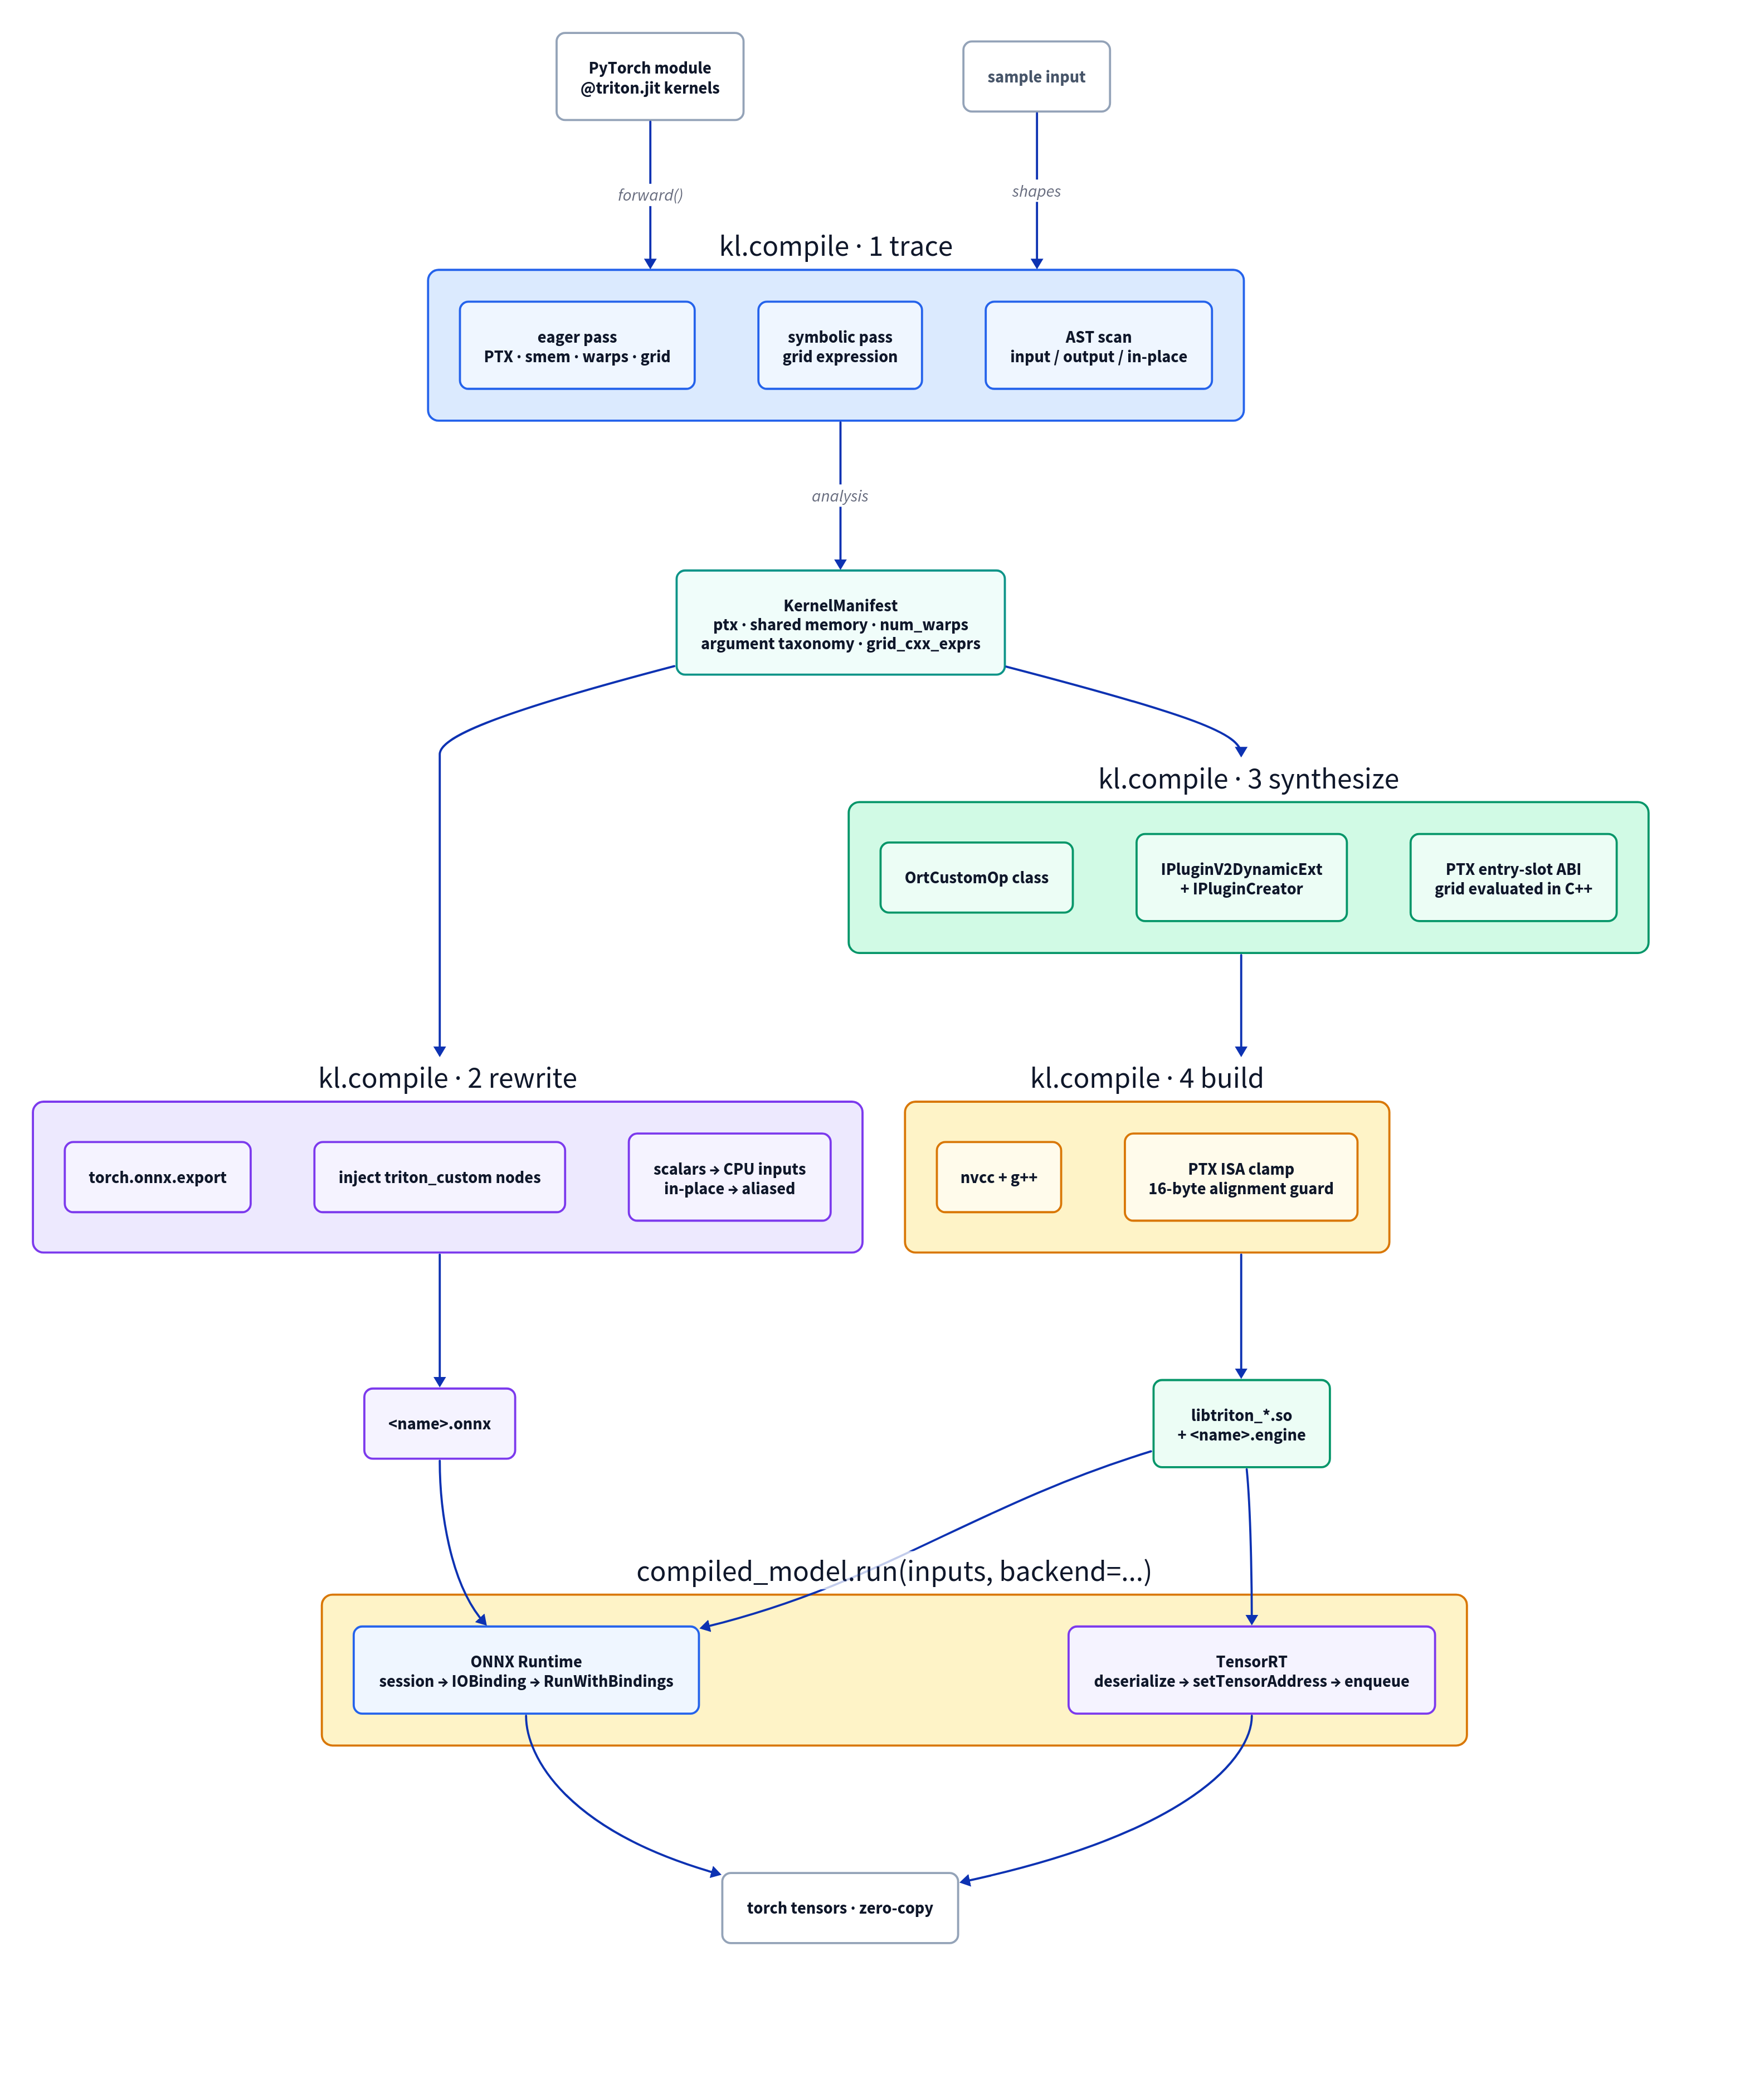
\includegraphics[width=0.56\textwidth]{pipeline_end_to_end.png}
\caption{The compile pipeline. Trace recovers the contract into a
\texttt{KernelManifest}; rewrite injects \texttt{triton\_custom} nodes into the
ONNX graph; synthesize emits the ONNX Runtime and TensorRT classes, rebuilding the
PTX entry-slot ABI and evaluating the grid in C++; build compiles the libraries.
The same artifacts drive both run lanes.}
\label{fig:compile}
\end{figure*}

\paragraph{Graph rewriting.} A hook inside \texttt{torch.onnx.export} replaces
each Triton launch with a custom-domain node
\texttt{triton\_custom::<kernel>} carrying the PTX and the taxonomy. Per-call
scalars become CPU inputs, so a new value needs no recompilation; in-place buffers
are wired input-to-output so the optimiser sees the mutation. Crucially, the node
is injected \emph{into} the graph, so TensorRT and ONNX Runtime still fold and
tune the surrounding standard layers.

\paragraph{Plugin synthesis.} For each kernel KernelLens emits an
\texttt{OrtCustomOp} class and a \texttt{nvinfer1::IPluginV2DynamicExt} plus
\texttt{IPluginCreator}. Both reconstruct the launch argument array from the
recovered ABI and evaluate the grid expression in C++ over the runtime
dimensions, so one compiled plugin serves dynamic shapes. A build step compiles
the sources and hardens the result: PTX ISA versions are clamped on load failure
for older driver JITs, and a 16-byte alignment guard stages sub-aligned tensor
slices through an aligned buffer.

\paragraph{Run.} \texttt{compiled\_model.run(inputs, backend=...)} loads the
library and hands PyTorch's GPU addresses straight to the engine
(Figure~\ref{fig:run}). ONNX Runtime: create the session, bind raw CUDA pointers
through \texttt{IOBinding}, \texttt{run\_with\_iobinding}. TensorRT: deserialize
into an \texttt{IExecutionContext}, \texttt{set\_tensor\_address} for every
tensor, \texttt{execute\_async\_v3}. Both cost $O(1)$ pointer registration plus
the kernel, versus $O(N)$ host staging copies.

\begin{figure*}[t]
\centering
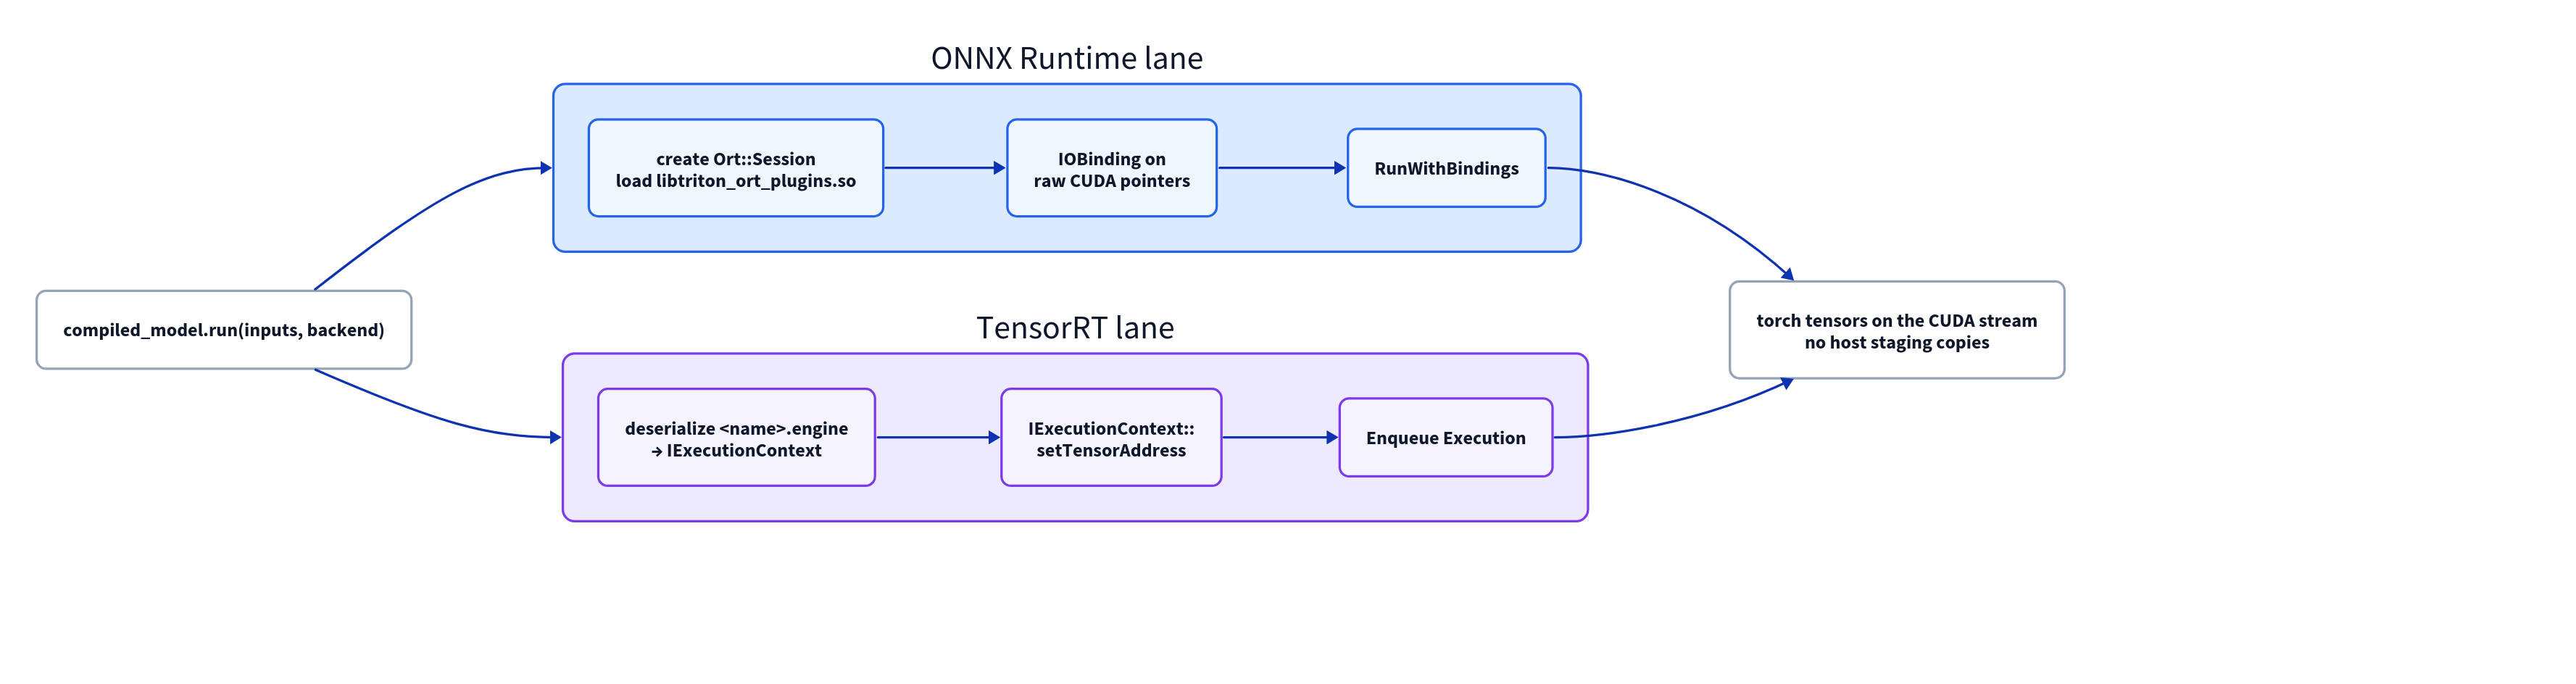
\includegraphics[width=\textwidth]{run_pipeline.png}
\caption{The run pipeline. One run call dispatches to either lane; neither moves
tensor data through the host.}
\label{fig:run}
\end{figure*}

\FloatBarrier
\section{Implementation and Code Comparison}
\label{sec:impl}

KernelLens is a Python package. The compiler is five modules---tracing, AST
analysis, manifest assembly, ONNX export, and the two code generators---and the
runtime is a single \texttt{CompiledModel} that dispatches to ONNX Runtime or
TensorRT. The user writes no C++.

The clearest way to convey what the framework does is to compare the two sides of
the same task: one fused RMSNorm kernel, running as a native operator in both
engines.

\paragraph{With KernelLens.} Listing~\ref{lst:kl} is the entire deployment. The
kernel and module are the ones the user already wrote.

\begin{lstlisting}[caption={The KernelLens side: two calls.},label={lst:kl},language=Python]
import kernel_lens as kl

compiled = kl.compile(
    RMSNorm(4096).cuda(), (x,),
    name="llama3_rmsnorm",
    backends=["onnx", "tensorrt"],
)
out_ort = compiled.run((x,), backend="onnx")
out_trt = compiled.run((x,), backend="tensorrt")
\end{lstlisting}

\paragraph{Without KernelLens.} Listing~\ref{lst:manual} is the shape of what you
write instead: a CUDA port of the kernel, an \texttt{OrtCustomOp}, a TensorRT
plugin and its creator, a build, a graph patch, and the engine-driving code.

\begin{lstlisting}[caption={The manual side: classes, build and engine calls you own.},label={lst:manual},language=C++]
// 1. port the kernel to CUDA                       (rmsnorm.cu)
// 2. ONNX Runtime custom operator
struct RmsnormOp : Ort::CustomOpBase<...> {
    const char* GetName() const { return "rmsnorm"; }
    ONNXTensorElementDataType GetInputType(size_t i) const;
    // ... plus a Compute() that rebuilds the PTX argument array
};
// 3. TensorRT plugin + creator
class RmsnormPlugin : public nvinfer1::IPluginV2DynamicExt {
    DimsExprs getOutputDimensions(...) noexcept override;
    bool supportsFormatCombination(...) noexcept override;
    int32_t enqueue(...) noexcept override;         // launch
    size_t getSerializationSize() const noexcept override;
    void serialize(void*) const noexcept override;
    IPluginV2DynamicExt* clone() const noexcept override;
};
class RmsnormPluginCreator : public nvinfer1::IPluginCreator { /* ... */ };
// 4. CMakeLists.txt, nvcc, g++, header resolution
// 5. a PyTorch C++ extension that patches the FX graph
//    and wraps each kernel with @torch.library.custom_op
// 6. drive the engines
//    Ort::Session + Ort::Binding + RunWithBindings
//    IExecutionContext + setTensorAddress + Enqueue Execution
\end{lstlisting}

\paragraph{Measured volume.} Table~\ref{tab:loc} counts the generated artifacts
for this one kernel, compiled for both backends. It is $\approx 1{,}329$ lines of
C++ across six files---before CMake, the FX-graph patch, or the engine-driving
code.

\begin{table*}[t]
\centering
\small
\begin{tabular}{l r l}
\toprule
\textbf{Artifact} & \textbf{Lines} & \textbf{Author} \\ \midrule
\texttt{ort\_plugins/<kernel>Op.cu} & 909 & hand, without KernelLens \\
\texttt{ort\_plugins/<kernel>Op.h} & 63 & hand \\
\texttt{ort\_plugins/register\_ops.cpp} & 25 & hand \\
\texttt{trt\_plugins/<kernel>Plugin.h} & 112 & hand \\
\texttt{trt\_plugins/<kernel>Plugin.cu} & $\approx$300 & hand \\
\texttt{trt\_plugins/register\_plugins.cpp} & $\approx$30 & hand \\ \midrule
\textbf{Total, one kernel} & $\mathbf{\approx 1{,}329}$ & \textbf{KernelLens: 0} \\
\bottomrule
\end{tabular}
\caption{Generated C++ volume for a single fused RMSNorm kernel, both backends,
measured with \texttt{tests/measure\_codegen.py}.}
\label{tab:loc}
\end{table*}

\section{Evaluation}
\label{sec:eval}

\subsection{Experimental setup}

All measurements are on a single NVIDIA GeForce RTX 5060~Ti (16~GB, Blackwell,
\texttt{sm\_120a}) with driver 570.144, CUDA~12.8, PyTorch~2.14.0, Triton~3.8.0,
ONNX Runtime~1.30.0 and TensorRT~10.16.1.11. Timings use CUDA events after
warm-up. Parity is measured against native Triton execution of the same kernel,
which isolates the recovered plumbing from the arithmetic.

The conformance, parity and real-model results are additionally reproduced on a
second architecture: an NVIDIA A100-SXM4-80GB (Ampere, \texttt{sm\_80}) with
driver 595.91, CUDA~13.3, PyTorch~2.8.0, Triton~3.4.0, ONNX
Runtime~1.31.0 and TensorRT~10.16.1.11. Table~\ref{tab:real} is measured on
that configuration. Results are reported per configuration and never blended
across them.

\subsection{Numerical parity}

\begin{table*}[t]
\centering
\small
\begin{tabular}{lcc}
\toprule
\textbf{Workload} & \textbf{ORT} & \textbf{TRT} \\ \midrule
LLaMA 3 / Mistral fused RMSNorm & $0.00\text{e}{+}00$ & $0.00\text{e}{+}00$ \\
Liger / PaLM SwiGLU & $0.00\text{e}{+}00$ & $0.00\text{e}{+}00$ \\
LLaMA 3 / Qwen 2.5 RoPE & $0.00\text{e}{+}00$ & $0.00\text{e}{+}00$ \\
Liger fused softmax + cross-entropy & $0.00\text{e}{+}00$ & $0.00\text{e}{+}00$ \\
Fused residual + RMSNorm & $\le 9.5\text{e}{-}07$ & $\le 9.5\text{e}{-}07$ \\
Mamba SSM recurrence & $4.8\text{e}{-}07$ & $4.8\text{e}{-}07$ \\
FP8 scaled GEMM / INT4 W4A16 GEMM & $0.00\text{e}{+}00$ & --- \\
Multi-output rank-4/3 log-sum-exp & $0.00\text{e}{+}00$ & $0.00\text{e}{+}00$ \\
In-place mutation (fp32 / fp16) & $0.00\text{e}{+}00$ & $0.00\text{e}{+}00$ \\
\bottomrule
\end{tabular}
\caption{Maximum absolute difference versus native Triton.}
\label{tab:parity}
\end{table*}

\subsection{Coverage of module patterns}

Parity on chosen operators is necessary but not sufficient: the recovery has to
work for the ways a module actually calls a kernel. A conformance suite exercises
fourteen patterns against both backends, all at $0.00\text{e}{+}00$: two kernels
in one graph; the same kernel launched twice with different scalars (each launch
receives its own operator and plugin); multiple outputs of different shapes;
dynamic host scalars; strided and dynamic-shape inputs; kernels inside a Python
loop and behind a conditional; kernels delegating to nested helpers; in-place
mutation; a 3-D launch grid; and fp16 and bf16 tensors. The one boundary is dtype
coverage on ONNX Runtime, which cannot bind a bfloat16 tensor to a custom
operator; bf16 models use TensorRT, which handles them exactly.

\subsection{Folding plus kernels}

This is the payoff of injecting the operator \emph{into} the graph. We take a
two-layer block whose attention is a custom squared-ReLU flash kernel, whose
normalisations and gated activation are custom kernels, and whose projections and
residuals are standard operators. It can be run three ways.

\begin{table*}[t]
\centering
\small
\begin{tabular}{lc c}
\toprule
\textbf{Configuration} & \textbf{Latency (ms)} & \textbf{Relative} \\ \midrule
A. Folded only --- eager, standard ops & $28.04$ & $0.54\times$ \\
A. Folded only --- \texttt{torch.compile} & $15.15$ & $1.00\times$ \\ \midrule
B. Kernels only --- eager Triton & $8.24$ & $1.84\times$ \\
B. Kernels only --- \texttt{torch.compile} & $7.55$ & $2.01\times$ \\ \midrule
C. KernelLens --- ONNX Runtime & $9.27$ & $1.63\times$ \\
\textbf{C. KernelLens --- TensorRT} & $\mathbf{7.63}$ & $\mathbf{1.99\times}$ \\
\bottomrule
\end{tabular}
\caption{Two-layer block, $D{=}512$, $H{=}8$, $S{=}4096$, batch 1. Relative is
versus the folded-only \texttt{torch.compile} row.}
\label{tab:folding}
\end{table*}

KernelLens runs the block in $7.63$~ms: $1.99\times$ faster than the folded-only
formulation and $3.68\times$ faster than eager folding, because folding has to
materialise the $O(N^2)$ attention that the kernel avoids; and $1.08\times$ faster
than the unfused kernel path, because the engine folds the standard layers around
it. The two halves are complementary, and KernelLens is the only configuration
that has both.

\subsection{Single-operator latency}

\begin{table*}[t]
\centering
\small
\resizebox{\textwidth}{!}{%
\begin{tabular}{lcccc}
\toprule
\textbf{Operator} & \textbf{PyTorch Eager} & \textbf{torch.compile} & \textbf{Native Triton} & \textbf{KernelLens ORT} \\ \midrule
LLaMA 3 RMSNorm (4,512,4096) & $0.517$ ms & $0.173$ ms & $\mathbf{0.160}$ ms & $0.172$ ms \\
PaLM SwiGLU (2048$\times$4096) & $0.429$ ms & $0.252$ ms & $\mathbf{0.252}$ ms & $0.270$ ms \\
Qwen 2.5 RoPE (4,512,32,128) & $0.673$ ms & $0.174$ ms & $\mathbf{0.159}$ ms & $0.180$ ms \\
Fused cross-entropy (32,32000) & $0.013$ ms & $0.013$ ms & $\mathbf{0.010}$ ms & $0.026$ ms \\
\bottomrule
\end{tabular}%
}
\caption{Single-operator latency. The C++ operator runs the same kernel within
6--13\% of native Triton on the larger operators; the value is deployment.}
\label{tab:micro}
\end{table*}

\subsection{End-to-end}

\begin{table*}[t]
\centering
\small
\resizebox{\textwidth}{!}{%
\begin{tabular}{lcccc}
\toprule
\textbf{Configuration} & \textbf{TTFT ($S{=}512$)} & \textbf{ITL ($S{=}1$)} & \textbf{Total (128 tok)} & \textbf{Peak VRAM} \\ \midrule
PyTorch Eager + Triton & $7.85$ ms & $0.866$ ms & $0.118$ s & $478.0$ MB \\
torch.compile (Inductor) & $7.92$ ms & $0.866$ ms & $0.118$ s & $473.0$ MB \\
KernelLens C++ plugins (ORT) & $4.37$ ms & $0.999$ ms & $0.131$ s & $464.2$ MB \\
\textbf{KernelLens TensorRT plugin} & $\mathbf{4.14}$ ms & $0.905$ ms & $0.119$ s & $466.2$ MB \\
\bottomrule
\end{tabular}%
}
\caption{End-to-end 4-layer LLaMA decoder ($D{=}1024$). The TensorRT plugin nearly
halves time-to-first-token and attains the lowest peak VRAM.}
\label{tab:e2e}
\end{table*}

\subsection{Quantized kernels}

\begin{table*}[t]
\centering
\small
\resizebox{\textwidth}{!}{%
\begin{tabular}{lcccc}
\toprule
\textbf{Kernel} & \textbf{Eager FP16} & \textbf{Native Triton} & \textbf{KL ORT} & \textbf{Speedup} \\ \midrule
FP8 scaled GEMM (4096$\times$4096) & $2.786$ ms & $2.046$ ms & $2.083$ ms & $1.34\times$ \\
INT4 W4A16 GEMM (2048$\times$4096) & $1.388$ ms & $3.570$ ms & $3.629$ ms & $0.38\times$ ($2\times$ smaller) \\
\bottomrule
\end{tabular}%
}
\caption{Quantized GEMMs on \texttt{sm\_120a}, where PTX ISA clamping is
exercised. Both reach exact parity with native Triton.}
\label{tab:quant}
\end{table*}

\subsection{Real pretrained models}

The models above are controlled PyTorch modules, which keeps the plumbing
comparable but leaves open whether the approach scales to a model people
actually serve. We therefore take real pretrained OPT checkpoints, replace every
\texttt{LayerNorm} in the decoder with the Triton RMSNorm kernel above
(carrying the weight across), and compile the result. OPT is used because its
architecture is exportable through the TorchScript path the compiler relies on;
the rotary-embedding families are not, and that is a property of the ONNX
exporter rather than of the recovered contract, since plain
\texttt{torch.onnx.export} fails on them identically.

\begin{table*}[t]
\centering
\footnotesize
\begin{tabular}{llrrrr}
\toprule
Model & dtype & Eager & \texttt{torch.compile} & ORT & TensorRT \\
\midrule
OPT-125M & fp32 & 12.1\,ms & 10.9\,ms & 4.8\,ms & \textbf{3.4}\,ms \\
OPT-125M & fp16 & 5.7\,ms & 2.4\,ms & 3.6\,ms & \textbf{2.0}\,ms \\
OPT-1.3B & fp32 & 98.6\,ms & 88.0\,ms & 23.4\,ms & \textbf{19.0}\,ms \\
OPT-1.3B & fp16 & 14.7\,ms & 10.8\,ms & 15.6\,ms & \textbf{9.9}\,ms \\
OPT-2.7B & fp32 & 175.9\,ms & 172.7\,ms & 37.4\,ms & \textbf{31.7}\,ms \\
OPT-2.7B & fp16 & 22.2\,ms & 17.5\,ms & 22.6\,ms & \textbf{16.5}\,ms \\
OPT-6.7B & fp16 & 37.0\,ms & 33.8\,ms & 40.2\,ms & \textbf{31.1}\,ms \\
\bottomrule
\end{tabular}
\caption{Real pretrained OPT checkpoints with every decoder
\texttt{LayerNorm} replaced by the Triton RMSNorm kernel. Prefill latency,
$S{=}512$, on an A100-SXM4-80GB. \texttt{torch.compile} is the meaningful
baseline: it captures the same kernels rather than reimplementing them. Bold
marks the fastest configuration, which is TensorRT at every size and precision.}
\label{tab:real}
\end{table*}

TensorRT is the fastest configuration throughout, but the comparison that
matters is against \texttt{torch.compile} rather than eager, since it captures
the same Triton kernels and differs only in how the surrounding operators are
scheduled. The picture splits by precision.

In fp32 \texttt{torch.compile} barely improves on eager ($1.02$--$1.12\times$)
because it does not fuse the operators around the kernel, whereas KernelLens
does: TensorRT is $3.18\times$, $4.62\times$ and $5.45\times$ faster than
\texttt{torch.compile} on 125M, 1.3B and 2.7B, and the margin grows with model
size. That growth is the graph-level fusion at work, not the normalisation
kernels.

In fp16 the ordering reverses. \texttt{torch.compile} then optimises well
($2.4\times$ over eager at 125M), and KernelLens only matches it: TensorRT
edges \texttt{torch.compile} by $1.06$--$1.22\times$ across all four sizes,
while ONNX Runtime is consistently \emph{slower} ($0.67$--$0.84\times$). The
compiled fp16 graph for OPT-125M carries $1{,}583$ nodes ($76$ \texttt{Cast},
$345$ \texttt{Unsqueeze}, $549$ \texttt{Constant}) against $25$ custom
operators, so per-node dispatch overhead dominates at these shapes.

Keeping kernels therefore pays only when the surrounding graph is left unfused.
When the baseline already fuses, it breaks even, and we do not claim otherwise.

Numerical agreement tracks precision rather than speed. In fp32 every model
retains the same argmax on at least $98.8\%$ of positions and the mean absolute
logit difference stays below $6.3\times10^{-3}$; OPT-350M in fp16 under ONNX
Runtime is bit-exact. Under TensorRT in fp16, agreement falls to
$93.4$--$97.9\%$ with a mean difference of up to $5.3\times10^{-2}$.

\section{Discussion}

\paragraph{When the engine wins, and when it does not.} TensorRT is not
universally faster than \texttt{torch.compile}, and we report both directions. On
GEMM-heavy transformer prefill the TensorRT plugin is $1.9\times$ faster ($4.14$
versus $7.92$~ms). On a convolution-heavy graph with a custom kernel it is behind,
even after fixing a dtype-promotion bug and declaring channel-last formats for
pointwise kernels; the remaining gap is the engine's convolution performance
rather than the plugin.

\paragraph{Why an engine at all.} The reasons are structural as much as
numerical: no Python interpreter and no \texttt{libtorch} in the serving path (no
GIL, a small footprint, deployable from non-Python services); a serialized engine
that cold-starts without recompiling; engine-level VRAM planning ($464$~MB versus
$473$/$478$~MB in our decoder); dynamic shapes handled by optimisation profiles
rather than recompiles and guards; and quantized inference, where TensorRT is
mature. The folding result is the numerical case: if the kernel cannot be shipped
at all, the folded-only formulation is $2\times$ slower.

\section{Threats to Validity}
\label{sec:threats}

\paragraph{Internal validity.} All timings are CUDA-event measurements on one
machine and one GPU. The folding comparison is sensitive to precision: an early
version of it showed a larger gap that was mostly TensorRT's default TF32 rather
than folding, and we enable TF32 in the PyTorch baselines to remove that
confound. Parity is measured against native Triton of the same kernel, which
isolates the plumbing from the arithmetic but does not certify the kernel itself
against a reference implementation.

\paragraph{External validity.} The evaluation spans two architectures (Blackwell
consumer and Ampere datacenter) but a single vendor, a single driver per
architecture, and fp32/fp16/bf16/FP8/INT4 on Blackwell. The absolute numbers do
not transfer to other GPUs or to distributed serving, and the "engine wins on
prefill" conclusion is specific to the shapes tested.

\paragraph{Construct validity.} "Coverage" is demonstrated by fourteen module
patterns, which is a strong sample but not a proof of universality; genuinely
exotic cases (custom \texttt{autograd.Function} kernels, CUDA-graph capture,
collectives inside a kernel's forward) are untested.

\section{Limitations and Future Work}

ONNX Runtime cannot bind bfloat16 to a custom operator, so bf16 models use
TensorRT. TensorRT's tensor path required routing INT8 and in-place-aliased
operators to the exact ONNX Runtime plugin. The generated ONNX Runtime registrar
exports a fixed symbol, so several compiled models that share a kernel base name
can interfere when loaded in one process. Future work: auto-tuning dispatch
(folding \texttt{@triton.autotune} variants into one plugin with a shape-keyed
table); CUDA-graph capture of the launch sequence; channel-last formats for
non-pointwise kernels; distributed execution with embedded NCCL handles; and a
Blackwell backend (cluster-launch descriptors, \texttt{cp.async.bulk}, NVFP4).

\paragraph{Engine coverage beyond ONNX.}
The recovered contract is engine-agnostic: it describes how a compiled Triton
kernel maps onto an engine's tensors, and only the injection step is
engine-specific. TensorRT-LLM is the natural next target, being the standard
way to serve LLMs on NVIDIA hardware. Its plugins \emph{are} TensorRT plugins
--- the same \texttt{IPluginV2DynamicExt} and \texttt{IPluginCreator}
interfaces generated here --- so the plugin generator carries over almost
unchanged, and TensorRT-LLM ships no automatic plugin generator of its own. The
work is consequently in the graph injection rather than the plugin:
TensorRT-LLM builds its engine from a checkpoint or from its own module API
rather than from an arbitrary ONNX graph, so the rewriting pass has no direct
equivalent and a new injection point is required. The reachable scope is
non-attention kernels --- normalisations, activations, fused elementwise ---
because TensorRT-LLM's attention plugin owns the paged KV cache, the
grouped-query mapping and in-flight batching, a contract a user kernel cannot
re-enter without reimplementing it.

\section{Conclusion}

A compiled Triton kernel is a self-contained artifact, but the interface between
it and a C++ engine is implicit. We showed that the interface can be recovered
automatically---the PTX entry signature, the symbolic launch grid, and the
argument taxonomy---and re-established as native TensorRT and ONNX Runtime
operators injected into the graph. The composition is exact on the research
kernels and fourteen module patterns, it replaces $1{,}137$ lines of
hand-written C++ per kernel with two Python calls, and it pays off: keeping the
kernel while letting the engine fold the rest is $1.99\times$ faster than the
folded-only formulation and $1.08\times$ faster than the unfused kernel path.

\section{Reproducibility Statement}

KernelLens is released as a Python package on PyPI (\texttt{pip install
kernel-lens}). The
evaluation scripts are in \texttt{tests/}: \texttt{test\_conformance.py} (the
fourteen module patterns), \texttt{test\_research\_kernels.py} (parity),
\texttt{benchmark\_folding\_vs\_triton.py} (the folding comparison),
\texttt{benchmark\_research\_kernels.py} and \texttt{benchmark\_e2e\_llama.py}
(latency and end-to-end), \texttt{test\_fp8\_gemm.py} and
\texttt{test\_int4\_dequant\_gemm.py} (quantized), and
\texttt{measure\_codegen.py} (the code-volume measurement). Raw measurements are
committed as JSON under \texttt{docs/assets/data/}. The complete source tree, the
evaluation scripts and the raw measurement JSON are provided as supplementary
material (\texttt{kernel\_lens\_supplementary.zip}). All results were produced on
the single RTX 5060~Ti configuration described in \S\ref{sec:eval}.

\FloatBarrier
\begin{thebibliography}{99}
\bibitem{triton2019} P. Tillet, H. Kung, and D. Cox, ``Triton: an intermediate language and compiler for tiled neural network computations,'' in \textit{ARRAY}, 2019.
\bibitem{llama3} AI@Meta, ``The Llama 3 Herd of Models,'' \textit{arXiv:2407.21783}, 2024.
\bibitem{ligerkernel} LinkedIn Corp., ``Liger-Kernel: Efficient Triton Kernels for LLM Training,'' 2024.
\bibitem{qwen25} Qwen Team, ``Qwen2.5 Technical Report,'' \textit{arXiv:2412.15115}, 2024.
\bibitem{flashattn1} T. Dao et al., ``FlashAttention: Fast and Memory-Efficient Exact Attention with IO-Awareness,'' in \textit{NeurIPS}, 2022.
\bibitem{flashattn2} T. Dao, ``FlashAttention-2,'' in \textit{ICLR}, 2024.
\bibitem{pytorch} A. Paszke et al., ``PyTorch: An imperative style, high-performance deep learning library,'' in \textit{NeurIPS}, 2019.
\bibitem{pytorch20} J. Ansel et al., ``PyTorch 2.0: TorchDynamo and TorchInductor,'' in \textit{ASPLOS}, 2024.
\bibitem{aotinductor} PyTorch Engineering Team, ``PyTorch AOTInductor,'' 2023.
\bibitem{tvm} T. Chen et al., ``TVM: An Automated End-to-End Optimizing Compiler for Deep Learning,'' in \textit{OSDI}, 2018.
\bibitem{mlir} C. Lattner et al., ``MLIR: Scaling Compiler Infrastructure for Domain Specific Architectures,'' in \textit{CGO}, 2021.
\bibitem{halide} J. Ragan-Kelley et al., ``Halide: A Language and Compiler for Optimizing Parallel Image Processing Pipelines,'' in \textit{PLDI}, 2013.
\bibitem{vllm} W. Kwon et al., ``Efficient Memory Management for LLM Serving with PagedAttention,'' in \textit{SOSP}, 2023.
\bibitem{tensorrt_llm} NVIDIA Corporation, ``TensorRT-LLM,'' \url{https://developer.nvidia.com/tensorrt}, 2023.
\bibitem{onnxruntime} Microsoft Corporation, ``ONNX Runtime,'' \url{https://onnxruntime.ai}, 2021.
\bibitem{tensorrt} NVIDIA Corporation, ``NVIDIA TensorRT,'' \url{https://developer.nvidia.com/tensorrt}, 2023.
\end{thebibliography}

\section*{AI Usage Disclosure}

An AI coding assistant (DeepSeek~V4.1~Flash, driven through OpenCode) was used
extensively in producing this work, and the authors take full responsibility
for all content. It was used for: (i)~implementing and debugging parts of the
\texttt{kernel\_lens} package, including the PTX entry-signature recovery, the
ONNX graph rewriting and the TensorRT and ONNX~Runtime code generators;
(ii)~writing the evaluation and regression scripts under \texttt{tests/};
(iii)~producing the diagrams and result figures and the project website;
(iv)~executing the benchmarks on the GPU host and tabulating the measurements;
and (v)~drafting and editing the manuscript text, including the abstract, the
introduction, the related-work synthesis and the presentation of the results.
The literature search and the experimental design were performed by the author.
Every reported measurement was produced by executing the code on real hardware;
no result, citation or number was invented by a model. The author has verified
all claims, references and measurements.


\end{document}